\chapter{Einleitung} % 3 Seiten

Nachfolgend wird eine kurze Einführung in das Thema gegeben und die weitere Vorgehensweise erläutert.

\section{Gegenstand der Arbeit}

Diese Arbeit verwendet die Begriffe \emph{klassische} und \emph{sicherheitskritische} Bereiche zur Differenzierung zwischen Wirtschafts- und Unternehmensteilen die keinen erhöhten Sicherheitsbedarf haben und denen die explizit höhere Anforderungen bezüglich der Sicherheit haben (z. B. Kernkraftwerke, Luft- und Raumfahrtindustrie).
Die Verletzung dieser Ansprüche kann den Verlust streng vertraulicher Daten, Gefahr für Leib und Leben oder negative Auswirkungen für die Umwelt zur Folge haben.
Die Begriffe \emph{vertikale} und \emph{horizontale Evolution} (vgl. \autoref{fig:evolution}) werden im Kontext dieser Arbeit wie folgt definiert:
\emph{Vertikale Evolution} betrifft die Anwendung agiler Entwicklungsmethoden auf die Vereinigung von Entwicklung und Betrieb von Software (DevOps).
Dahingegen beschreibt \emph{horizontale Evolution} die Implementierung von agilen Vorgehensmodellen und Methoden in sicherheitskritischen Bereichen.

\begin{figure}
  \centering
  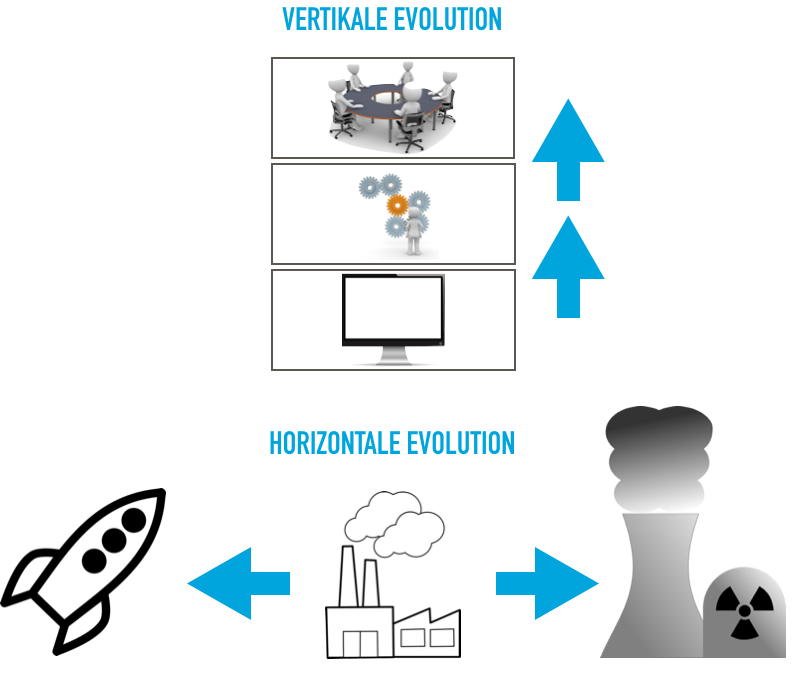
\includegraphics[width=\textwidth]{img/evolution.png}
  \caption{Vertikale und horizontale Evolution}
  \label{fig:evolution}
\end{figure}

Die agile Entwicklung ist nach diversen Studien und Umfragen bei den meisten Unternehmen im Alltag angekommen \parencite[vgl.][]{VersionOne:2015aa, HP:2015aa}. 
Damit hat sich der Trend fortgesetzt, von klassischen zu agilen Vorgehensmodellen über zu gehen \parencite[vgl.][]{Rodriguez:2012:SAL:2372251.2372275}.

Des Weiteren sind agile Vorgehensmodelle nicht nur auf die Entwicklung von Software beschränkt, sondern könnten auch auf den Betrieb von Software (DevOps) ausgeweitet werden.
Eine Fragestellung ist hierbei, welche Verbesserungen unter welchen Voraussetzungen durch die Anwendung von DevOps erreicht werden können und ob diese auch in sicherheitskritsichen Bereichen möglich sind.

In der gängigen Literatur wird meist nur auf die Anwendung von agilen Vorgehensmodellen in klassischen Bereichen eingegangen.
Insbesondere die sicherheitskritischen Bereiche, wie die Luft- und Raumfahrtindustrie, nutzen jedoch noch klassische Vorgehensmodelle.
Hier stellt sich die Frage, wie und ob diese Bereiche auch von den agilen Vorgehensmodellen profitieren können.

Die Relevanz der Fragestellung ergibt sich aus der Tatsache, dass gerade diese Bereiche oft unter hohen Lieferverzögerungen und Kostenüberschreitungen leiden.
Außerdem befindet sich beispielsweise die Raumfahrtindustrie in einem Wandel, da immer mehr private Unternehmen auf diesen Markt drängen, was einen erhöhten Wettbewerbsdruck verursacht.
Zwar finden sich zu den Themen agile Vorgehensmodelle und DevOps eine Vielzahl von Veröffentlichungen, jedoch nur sehr wenige beschäftigen sich mit der Anwendung und den Schwierigkeiten in sicherheitskritischen Bereichen.

\section{Zielsetzung}

Die vorliegende Arbeit soll untersuchen, wie und unter welchen Voraussetzungen sich DevOps einführen lässt und ob DevOps auch in sicherheitskritischen Bereichen Anwendung finden kann.
Außerdem soll geklärt werden, wie sich die Anwendung von agilen Vorgehensmodellen und deren Methoden auf sicherheitskritische Bereiche erweitern lässt.
Insbesondere soll untersucht werden, worin sich die klassischen und sicherheitskritischen Bereiche unterscheiden und welche Voraussetzungen geschaffen werden müssen, damit agile Methoden und DevOps eingeführt werden können.
Durch Betrachtung von Fallstudien, die die Einführung von DevOps und agilen Vorgehensmodellen in sicherheitskritischen Bereichen untersuchen, soll erarbeitet werden, welche Anpassungen an den Konzepten notwendig sind, um in diesen Bereichen sinnvoll eingesetzt werden zu können.
Abschließend sollen Schlussfolgerungen und Handlungsempfehlungen für sicherheitskritische Bereiche formuliert werden.


\section{Methodik}

Da die Arbeit bisherige Kenntnisse bezüglich sicherheitskritischen Bereichen, agilen Vorgehensmodellen und DevOps zusammentragen soll, bietet sich die Methode des \emph{Literatur-Reviews} \parencite[vgl.][]{Fettke:2006aa} an.
Somit kann der aktuelle Stand der Forschung erfasst und interpretiert werden.
Die grundlegenden Themen agile Entwicklung und DevOps finden sich in vielen Veröffentlichungen wieder, somit soll hierbei eine Komprimierung auf die wesentlichen, allgemein anerkannten Aspekte stattfinden.

\section{Gang der Untersuchung}

Die Arbeit beginnt mit einer umfassenden Einführung in die Grundlagen,
die klassische und agile Vorgehensmodelle vorstellt.
Anschließend wird der Begriff DevOps eingeführt.
Zur Erreichung der Ziele dieser Arbeit, werden \emph{klassische} und \emph{sicherheitskritische} Bereiche bezüglich dem Sicherheitsanspruch, den Normen, den konkreten Entwicklungspraktiken und der Time To Market verglichen.

Zur Suche wird auf die Quellen HTWG Bibliothek \parencite[vgl.][]{HTWG2015aa}, Google Scholar \parencite[vgl.][]{Google2015aa} und Google \parencite[vgl.][]{Google2015ab} zurückgegriffen.
Unter anderem werden die Stichwörter (und deren englische Entsprechung)
\begin{itemize}
\item Agile
\item Agile Entwicklung
\item Vorgehensmodelle
\item Sicherheitskritische Branchen
\item Luftfahrtindustrie
\item Raumfahrtindustrie
\item Luft- und Raumfahrt
\item Softwaresicherheit
\item Time to Market
\item Softwaresicherheit Anforderungen
\item Softwarenormen
\item DevOps Stichwörter HIER ERGÄNZEN
\end{itemize}
zur Literatursuche benutzt.
Diese werden in allem möglichen Kombinationen miteinander mit einem logischen Oder verknüpft.
Die gefundene Literatur dient als weitere Quelle für relevante Literatur, indem Zitate und Quellenverweise rückwärts durchsucht werden.

